% questions.tex —— 1995 年·全国卷·理科 · 题目内容片段（无答案）
% 由 tools/generate_projects.py 依来源总账自 1995/1995_数学真题_全国理_试题.md 生成，勿手改（改源 MD 后重跑）


\begin{gktip}
来源说明：本稿按固定来源单页 A3 扫描件转录，共 26 题（选择 1–15、填空 16–20、解答 21–26）。来源页\textbf{没有答案、解析与分值}，本卷答案由本项目独立推导并双人交叉核对（等级 D），不冒称官方答案。第 14 题源页选项（A）与（C）重复，已按原样保留并登记；第 23 题「点 E 在底面的圆周上」按源图取在下底面。

图形说明：第 2、5、15、23 题的 TikZ 图稿依原页拓扑重绘，不宣称按比例测绘。
\end{gktip}

\begin{gktip}
固定来源为单页横向 A3 试卷，印刷页码 51。按页面三栏顺序转录，共 26 题：1—15 选择题，16—20 填空题，21—26 解答题。来源页未载答案、解析、分值或总分；均不补造。本稿和四幅矢量示意图待独立核对，不是正式验收卷。
\end{gktip}

\begin{question}
\gkti{1}已知 $I$ 为全集，集合 $M,N\subseteq I$，若 $M\cap N=N$，则\mbox{（　　）}。

（A）$\overline{M}\supseteq\overline{N}$　　（B）$M\subseteq\overline{N}$　　（C）$\overline{M}\subseteq\overline{N}$　　（D）$M\supseteq\overline{N}$

\Needspace{0.4\textheight}
\end{question}
\begin{question}
\gkti{2}函数 $y=-\dfrac{1}{x+1}$ 的图象是\mbox{（　　）}。
\nopagebreak[4]
\begin{center}% 固定来源PDF印刷页51第2题四个图象选项的矢量示意重绘。
% 渐近线位置、分支象限及选项标签忠于原页；比例仅作示意。
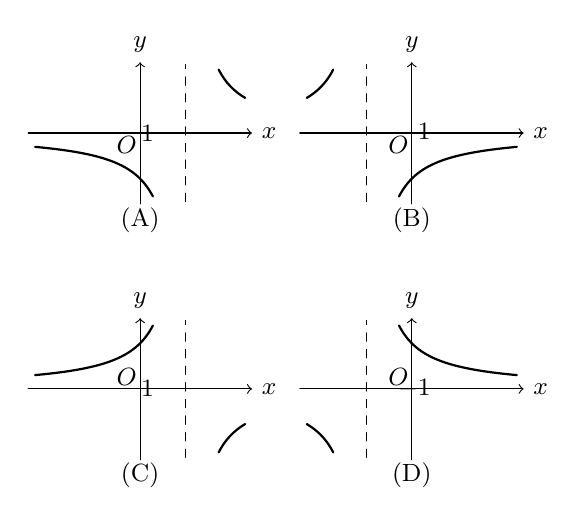
\begin{tikzpicture}[x=.58cm,y=.58cm,font=\small,line cap=round,line join=round]
  % (A) y=1/(x-1)
  \begin{scope}
    \draw[->] (-2.45,0)--(2.45,0) node[right] {$x$};
    \draw[->] (0,-1.55)--(0,1.55) node[above] {$y$};
    \draw[dashed] (1,-1.5)--(1,1.5);
    \draw[thick,domain=-2.3:.28,samples=60,variable=\x] plot (\x,{1/(\x-1)});
    \draw[thick,domain=1.72:2.3,samples=60,variable=\x] plot (\x,{1/(\x-1)});
    \node[left=8pt] at (1,0) {$1$};
    \node[below left,inner sep=1pt] at (0,0) {$O$};
    \node at (0,-1.9) {(A)};
  \end{scope}

  % (B) y=-1/(x+1), the graph of the stated function.
  \begin{scope}[xshift=3.45cm]
    \draw[->] (-2.45,0)--(2.45,0) node[right] {$x$};
    \draw[->] (0,-1.55)--(0,1.55) node[above] {$y$};
    \draw[dashed] (-1,-1.5)--(-1,1.5);
    \draw[thick,domain=-2.3:-1.72,samples=60,variable=\x] plot (\x,{-1/(\x+1)});
    \draw[thick,domain=-.28:2.3,samples=60,variable=\x] plot (\x,{-1/(\x+1)});
    \node[right=8pt] at (-1,0) {$-1$};
    \node[below left,inner sep=1pt] at (0,0) {$O$};
    \node at (0,-1.9) {(B)};
  \end{scope}

  % (C) y=-1/(x-1)
  \begin{scope}[yshift=-3.25cm]
    \draw[->] (-2.45,0)--(2.45,0) node[right] {$x$};
    \draw[->] (0,-1.55)--(0,1.55) node[above] {$y$};
    \draw[dashed] (1,-1.5)--(1,1.5);
    \draw[thick,domain=-2.3:.28,samples=60,variable=\x] plot (\x,{-1/(\x-1)});
    \draw[thick,domain=1.72:2.3,samples=60,variable=\x] plot (\x,{-1/(\x-1)});
    \node[left=8pt] at (1,0) {$1$};
    \node[above left,inner sep=1pt] at (0,0) {$O$};
    \node at (0,-1.9) {(C)};
  \end{scope}

  % (D) y=1/(x+1)
  \begin{scope}[xshift=3.45cm,yshift=-3.25cm]
    \draw[->] (-2.45,0)--(2.45,0) node[right] {$x$};
    \draw[->] (0,-1.55)--(0,1.55) node[above] {$y$};
    \draw[dashed] (-1,-1.5)--(-1,1.5);
    \draw[thick,domain=-2.3:-1.72,samples=60,variable=\x] plot (\x,{1/(\x+1)});
    \draw[thick,domain=-.28:2.3,samples=60,variable=\x] plot (\x,{1/(\x+1)});
    \node[right=8pt] at (-1,0) {$-1$};
    \node[above left,inner sep=1pt] at (0,0) {$O$};
    \node at (0,-1.9) {(D)};
  \end{scope}
\end{tikzpicture}
\end{center}
\nopagebreak[4]
\end{question}
\begin{question}
\gkti{3}函数
\nopagebreak[4]
\[
y=4\sin\left(3x+\frac\pi4\right)+3\cos\left(3x+\frac\pi4\right)
\]
的最小正周期是\mbox{（　　）}。

（A）$6\pi$　　（B）$2\pi$　　（C）$\dfrac{2\pi}{3}$　　（D）$\dfrac\pi3$

\end{question}
\begin{question}
\gkti{4}正方体的全面积是 $a^2$，它的顶点都在球面上，这个球的表面积是\mbox{（　　）}。

（A）$\dfrac{\pi a^2}{3}$　　（B）$\dfrac{\pi a^2}{2}$　　（C）$2\pi a^2$　　（D）$3\pi a^2$

\Needspace{0.4\textheight}
\end{question}
\begin{question}
\gkti{5}如图，若图中的直线 $l_1,l_2,l_3$ 的斜率分别为 $k_1,k_2,k_3$，则\mbox{（　　）}。
\nopagebreak[4]
\begin{center}% 固定来源PDF印刷页51第5题斜率关系示意重绘；仅保留线条的增减趋势。
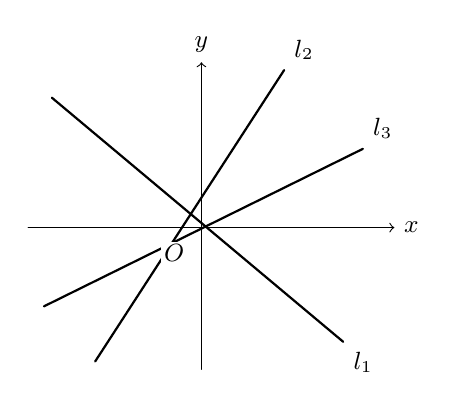
\begin{tikzpicture}[x=1cm,y=1cm,font=\small,line cap=round,line join=round]
  \draw[->] (-2.2,0)--(2.45,0) node[right] {$x$};
  \draw[->] (0,-1.8)--(0,2.1) node[above] {$y$};
  \draw[thick] (-1.9,1.65)--(1.8,-1.45) node[below right] {$l_1$};
  \draw[thick] (-1.35,-1.7)--(1.05,2.0) node[above right] {$l_2$};
  \draw[thick] (-2.0,-1.0)--(2.05,1.0) node[above right] {$l_3$};
  \node[fill=white,inner sep=1pt,below left=5pt] at (0,0) {$O$};
\end{tikzpicture}
\end{center}
\nopagebreak[4]
（A）$k_1<k_2<k_3$　　（B）$k_3<k_1<k_2$　　（C）$k_3<k_2<k_1$　　（D）$k_1<k_3<k_2$

\end{question}
\begin{question}
\gkti{6}在 $(1-x^3)(1+x)^{10}$ 的展开式中，$x^5$ 的系数是\mbox{（　　）}。

（A）$-297$　　（B）$-252$　　（C）$297$　　（D）$207$

\end{question}
\begin{question}
\gkti{7}使 $\arcsin x>\arccos x$ 成立的 $x$ 的取值范围是\mbox{（　　）}。

（A）$\left(0,\dfrac{\sqrt2}{2}\right]$　　（B）$\left(\dfrac{\sqrt2}{2},1\right]$　　（C）$\left[-1,\dfrac{\sqrt2}{2}\right)$　　（D）$[-1,0)$

\end{question}
\begin{question}
\gkti{8}双曲线 $3x^2-y^2=3$ 的渐近线方程是\mbox{（　　）}。

（A）$y=\pm3x$　　（B）$y=\pm\dfrac13x$　　（C）$y=\pm\sqrt3x$　　（D）$y=\pm\dfrac{\sqrt3}{3}x$

\end{question}
\begin{question}
\gkti{9}已知 $\theta$ 是第三象限角，且 $\sin^4\theta+\cos^4\theta=\dfrac59$，那么 $\sin2\theta$ 等于\mbox{（　　）}。

（A）$\dfrac{2\sqrt2}{3}$　　（B）$-\dfrac{2\sqrt2}{3}$　　（C）$\dfrac23$　　（D）$-\dfrac23$

\end{question}
\begin{question}
\gkti{10}已知直线 $l\perp$ 平面 $\alpha$，直线 $m\subset$ 平面 $\beta$，有下面四个命题：

① $\alpha\parallel\beta\Rightarrow l\perp m$；　② $\alpha\perp\beta\Rightarrow l\parallel m$；　③ $l\parallel m\Rightarrow\alpha\perp\beta$；　④ $l\perp m\Rightarrow\alpha\parallel\beta$。

其中正确的两个命题是\mbox{（　　）}。

（A）①与②　　（B）③与④　　（C）②与④　　（D）①与③

\end{question}
\begin{question}
\gkti{11}已知 $y=\log_a(2-ax)$ 在 $[0,1]$ 上是 $x$ 的减函数，则 $a$ 的取值范围是\mbox{（　　）}。

（A）$(0,1)$　　（B）$(1,2)$　　（C）$(0,2)$　　（D）$[2,+\infty)$

\end{question}
\begin{question}
\gkti{12}等差数列 $\{a_n\},\{b_n\}$ 的前 $n$ 项和分别为 $S_n$ 与 $T_n$，若
\nopagebreak[4]
\[
\frac{S_n}{T_n}=\frac{2n}{3n+1},
\]
则 $\displaystyle\lim_{n\to\infty}\frac{a_n}{b_n}$ 等于\mbox{（　　）}。

（A）$1$　　（B）$\dfrac{\sqrt6}{3}$　　（C）$\dfrac23$　　（D）$\dfrac49$

\end{question}
\begin{question}
\gkti{13}用 $1,2,3,4,5$ 这五个数字组成没有重复数字的三位数，其中偶数共有\mbox{（　　）}。

（A）24 个　　（B）30 个　　（C）40 个　　（D）60 个

\end{question}
\begin{question}
\gkti{14}在极坐标系中，椭圆的二焦点分别在极点和点 $(2c,0)$，离心率为 $e$，则它的极坐标方程是\mbox{（　　）}。

（A）$\rho=\dfrac{c(1-e)}{1-e\cos\theta}$　　（B）$\rho=\dfrac{c(1-e^2)}{1-e\cos\theta}$

（C）$\rho=\dfrac{c(1-e)}{1-e\cos\theta}$　　（D）$\rho=\dfrac{c(1-e^2)}{e(1-e\cos\theta)}$

\Needspace{0.4\textheight}
\end{question}
\begin{question}
\gkti{15}如图，$A_1B_1C_1-ABC$ 是直三棱柱，$\angle BCA=90^\circ$，点 $D_1,F_1$ 分别是 $A_1B_1,A_1C_1$ 的中点，若 $BC=CA=CC_1$，则 $BD_1$ 与 $AF_1$ 所成的角的余弦值是\mbox{（　　）}。
\nopagebreak[4]
\begin{center}% 固定来源PDF印刷页51第15题直三棱柱及指定线段的示意重绘。
% 仅表示标号、棱与中点关系，投影比例不代表题设长度。
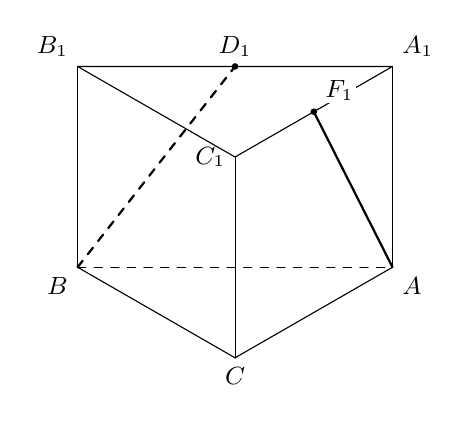
\begin{tikzpicture}[x=1cm,y=1cm,font=\small,line cap=round,line join=round]
  \coordinate (B) at (-2,0);
  \coordinate (A) at (2,0);
  \coordinate (C) at (0,-1.15);
  \coordinate (B1) at (-2,2.55);
  \coordinate (A1) at (2,2.55);
  \coordinate (C1) at (0,1.4);
  \coordinate (D1) at (0,2.55);
  \coordinate (F1) at (1,1.975);

  % Bottom triangle: the rear edge is hidden in the source projection.
  \draw[dashed] (B)--(A);
  \draw (B)--(C)--(A);
  % Top triangle and lateral edges of the right prism.
  \draw (B1)--(A1)--(C1)--cycle;
  \draw (B)--(B1) (A)--(A1) (C)--(C1);
  % The requested segments BD_1 and AF_1.
  \draw[dashed,thick] (B)--(D1);
  \draw[thick] (A)--(F1);

  \fill (D1) circle (1.2pt) (F1) circle (1.2pt);
  \node[above left] at (B1) {$B_1$};
  \node[above right] at (A1) {$A_1$};
  \node[left] at (C1) {$C_1$};
  \node[above] at (D1) {$D_1$};
  \node[fill=white,inner sep=1pt,above right=3pt] at (F1) {$F_1$};
  \node[below left] at (B) {$B$};
  \node[below right] at (A) {$A$};
  \node[below] at (C) {$C$};
\end{tikzpicture}
\end{center}
\nopagebreak[4]
（A）$\dfrac{\sqrt{30}}{10}$　　（B）$\dfrac12$　　（C）$\dfrac{\sqrt{30}}{15}$　　（D）$\dfrac{\sqrt{15}}{10}$

\end{question}
\begin{question}
\gkti{16}不等式
\nopagebreak[4]
\[
\left(\dfrac13\right)^{x^2-8}>3^{-2x}
\]
的解集是\underline{\qquad\qquad}。

\end{question}
\begin{question}
\gkti{17}已知圆台上、下底面圆周都在球面上，且下底面过球心，母线与底面所成的角为 $\dfrac\pi3$，则圆台的体积与球体积之比为\underline{\qquad\qquad}。

\end{question}
\begin{question}
\gkti{18}函数 $y=\sin\left(x-\dfrac\pi6\right)\cos x$ 的最小值是\underline{\qquad\qquad}。

\end{question}
\begin{question}
\gkti{19}直线 $l$ 过抛物线 $y^2=a(x+1)\quad(a>0)$ 的焦点，并且与 $x$ 轴垂直，若 $l$ 被抛物线截得的线段长为 $4$，则 $a=$\underline{\qquad\qquad}。

\end{question}
\begin{question}
\gkti{20}四个不同的小球放入编号为 $1,2,3,4$ 的四个盒中，则恰有一个空盒的放法共有\underline{\qquad\qquad}种（用数字作答）。

\end{question}
\begin{question}
\gkti{21}在复平面上，一个正方形的四个顶点按照逆时针方向依次为 $Z_1,Z_2,Z_3,O$（其中 $O$ 是原点），已知 $Z_2$ 对应复数 $Z_2=1+\sqrt3i$。求 $Z_1$ 和 $Z_3$ 对应的复数。

\end{question}
\begin{question}
\gkti{22}求 $\sin^2 20^\circ+\cos^2 50^\circ+\sin20^\circ\cos50^\circ$ 的值。

\Needspace{0.4\textheight}
\end{question}
\begin{question}
\gkti{23}如图，圆柱的轴截面 $ABCD$ 是正方形，点 $E$ 在底面的圆周上，$AF\perp DE$，$F$ 是垂足。
\nopagebreak[4]
\begin{center}% 固定来源PDF印刷页51第23题圆柱、轴截面和垂足的示意重绘。
% 图中比例仅作示意，不添加题干未给出的度量条件。
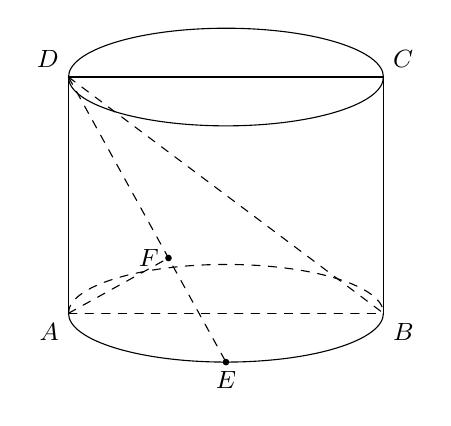
\begin{tikzpicture}[x=1cm,y=1cm,font=\small,line cap=round,line join=round]
  \coordinate (A) at (0,0);
  \coordinate (B) at (4,0);
  \coordinate (C) at (4,3);
  \coordinate (D) at (0,3);
  \coordinate (E) at (2,-.62);
  % F is the orthogonal projection of A onto DE in this schematic.
  \coordinate (F) at (1.269849,.701574);

  % Cylinder surface and circular rims; back half of the lower rim is hidden.
  \draw (D)--(A) (C)--(B);
  \draw (D)--(C);
  \draw (2,3) ellipse (2 and .62);
  \draw[dashed] (A) arc[start angle=180,end angle=0,x radius=2,y radius=.62];
  \draw (A) arc[start angle=180,end angle=360,x radius=2,y radius=.62];
  % Axial-section diagonal, DE and its perpendicular AF.
  \draw[dashed] (D)--(B);
  \draw[dashed] (A)--(B);
  \draw[dashed] (D)--(E) (A)--(F);
  \fill (E) circle (1.2pt) (F) circle (1.2pt);

  \node[above left] at (D) {$D$};
  \node[above right] at (C) {$C$};
  \node[below left] at (A) {$A$};
  \node[below right] at (B) {$B$};
  \node[below] at (E) {$E$};
  \node[left] at (F) {$F$};
\end{tikzpicture}
\end{center}
\nopagebreak[4]
（1）求证：$AF\perp DB$；

（2）如果圆柱与三棱锥 $D-ABE$ 的体积的比等于 $3\pi$，求直线 $DE$ 与平面 $ABCD$ 所成的角。

\end{question}
\begin{question}
\gkti{24}某地为促进淡水鱼养殖业的发展，将价格控制在适当范围内，决定对淡水鱼养殖提供政府补贴。设淡水鱼的市场价格为 $x$ 元/千克，政府补贴为 $t$ 元/千克。根据市场调查，当 $8\le x\le14$ 时，淡水鱼的市场日供应量 $P$ 千克与市场日需求量 $Q$ 千克近似满足关系：
\nopagebreak[4]
\[
P=1000(x+t-8)\quad(x\ge8,\ t\ge0),\qquad
Q=500\sqrt{40-(x-8)^2}\quad(8\le x\le14)
\]
当 $P=Q$ 时市场价格称为市场平衡价格。

（1）将市场平衡价格表示为政府补贴的函数，并求出函数的定义域；

（2）为使市场平衡价格不高于每千克 10 元，政府补贴至少为每千克多少元？

\end{question}
\begin{question}
\gkti{25}设 $\{a_n\}$ 是由正数组成的等比数列，$S_n$ 是其前 $n$ 项和。

\Needspace{5\baselineskip}
（1）证明：
\nopagebreak[4]
\[
\frac{\lg S_n+\lg S_{n+2}}{2}<\lg S_{n+1};
\]

\Needspace{5\baselineskip}
（2）是否存在常数 $c>0$，使得
\nopagebreak[4]
\[
\frac{\lg(S_n-c)+\lg(S_{n+2}-c)}{2}=\lg(S_{n+1}-c)
\]
成立？并证明你的结论。

\end{question}
\begin{question}
\gkti{26}已知椭圆 $\dfrac{x^2}{24}+\dfrac{y^2}{16}=1$，直线 $l$：$\dfrac{x}{12}+\dfrac{y}{8}=1$
\Needspace{5\baselineskip}
$P$ 是 $l$ 上一点，射线 $OP$ 交椭圆于点 $R$，又点 $Q$ 在 $OP$ 上且满足
\nopagebreak[4]
\[
|OQ|\cdot|OP|=|OR|^2
\]
当点 $P$ 在 $l$ 上移动时，求点 $Q$ 的轨迹方程，并说明轨迹是什么曲线。

\end{question}